\documentclass[a4paper,10pt]{article}
\usepackage[utf8]{inputenc}
\usepackage[english]{babel}
\usepackage[onehalfspacing]{setspace}
\usepackage{float}
\usepackage{biblatex}   % Using reference package
\addbibresource{mybibliography.bib}

\usepackage[nottoc]{tocbibind} %Adds "References" to the table of contents
\usepackage{graphicx}
\usepackage{hyperref}
%\graphicspath{/home/trung/Pictures/} \usepackage{float}
\hypersetup{
    colorlinks=true,
    linkcolor=blue,
    filecolor=magenta,      
    urlcolor=cyan,
}
%Document title, author and date (empty)
\title{Python Guideline for Beginner}
\author{Trung Nguyen}
\date{}

%Beginning of the document
\begin{document}

\maketitle

\tableofcontents

\section{Introduction}

In March 2020 python is the most popular programming languages were searches for tutorial by 31.17\% \href{http://pypl.github.io/PYPL.html}{PYPL}\cite{PYPL}.\newline
Anaconda is a free and open-source distribution of the Python programming languages which aims to simplify the package management and deployment. Anaconda work on Windows, Linux, and Mac OS and helps manage libraries, dependencies, and the environment. The virtual environment manager allowing you to install independent development environments and switch from one to the other (like virtualenv).\\ 
This document will guide the starter on how to set up the environment from scratch.\\
Skip the introduction part and start immediately by go to \hyperref[sec:start]{Getting started} section.


% ---------------------------------------------------------------------

\section{ Software Install}

This document only covers the scope of install the software base on Linux. However, the window installation is very similar(google on how to install Anaconda for window).\\
Download Anaconda from the official website:\href{https://www.anaconda.com/products/individual}{Anaconda}.\\
Select Linux and then Download the installer.Navigator is automatically installed when you install Anaconda version 4.0.0 or higher.If you have Miniconda or an older version of Anaconda installed, you can install Navigator from an Anaconda Prompt by running the command:" conda install anaconda-navigator ".\\
The Anaconda\_navigator user interface looks like the picture below:

\vspace{5mm}

\begin{figure}[H]
\centering
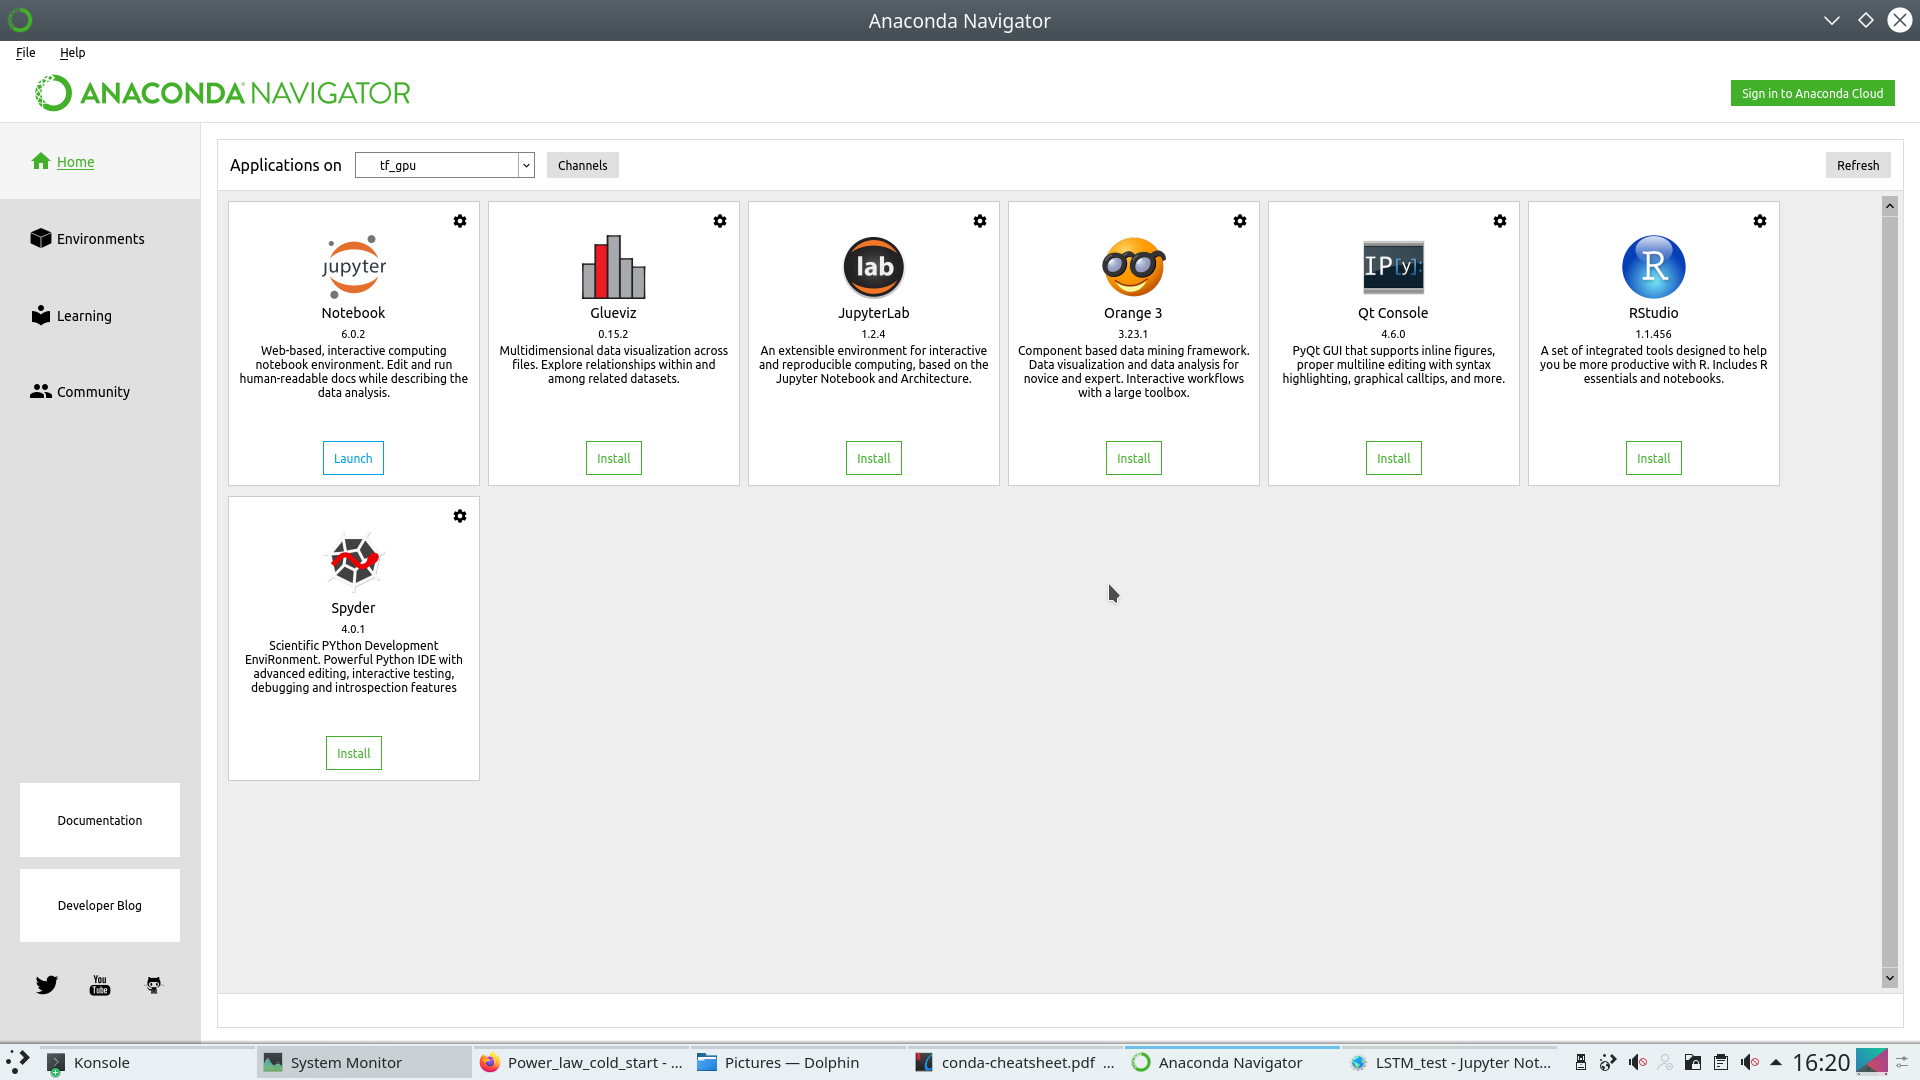
\includegraphics[width=1\columnwidth]{Anaconda_navigator.png}
\caption[Short title]{Anaconda navigator}
\label{fig:ff1}\end{figure}

\vspace{5mm}

Now you can install Jupyter notebook and Sypder for working with Python.\\
Download conda cheat-sheet (google with key word conda cheat sheet) to see how to create an virtual environment and activate it.\\
The link below give you more information on what is Anaconda and why do we use it:
\href{https://protostar.space/why-you-need-python-environments-and-how-to-manage-them-with-conda}{Anaconda}.\\
An alternative option is using Anaconda-navigator graphical interface.


\begin{figure}[H]
\centering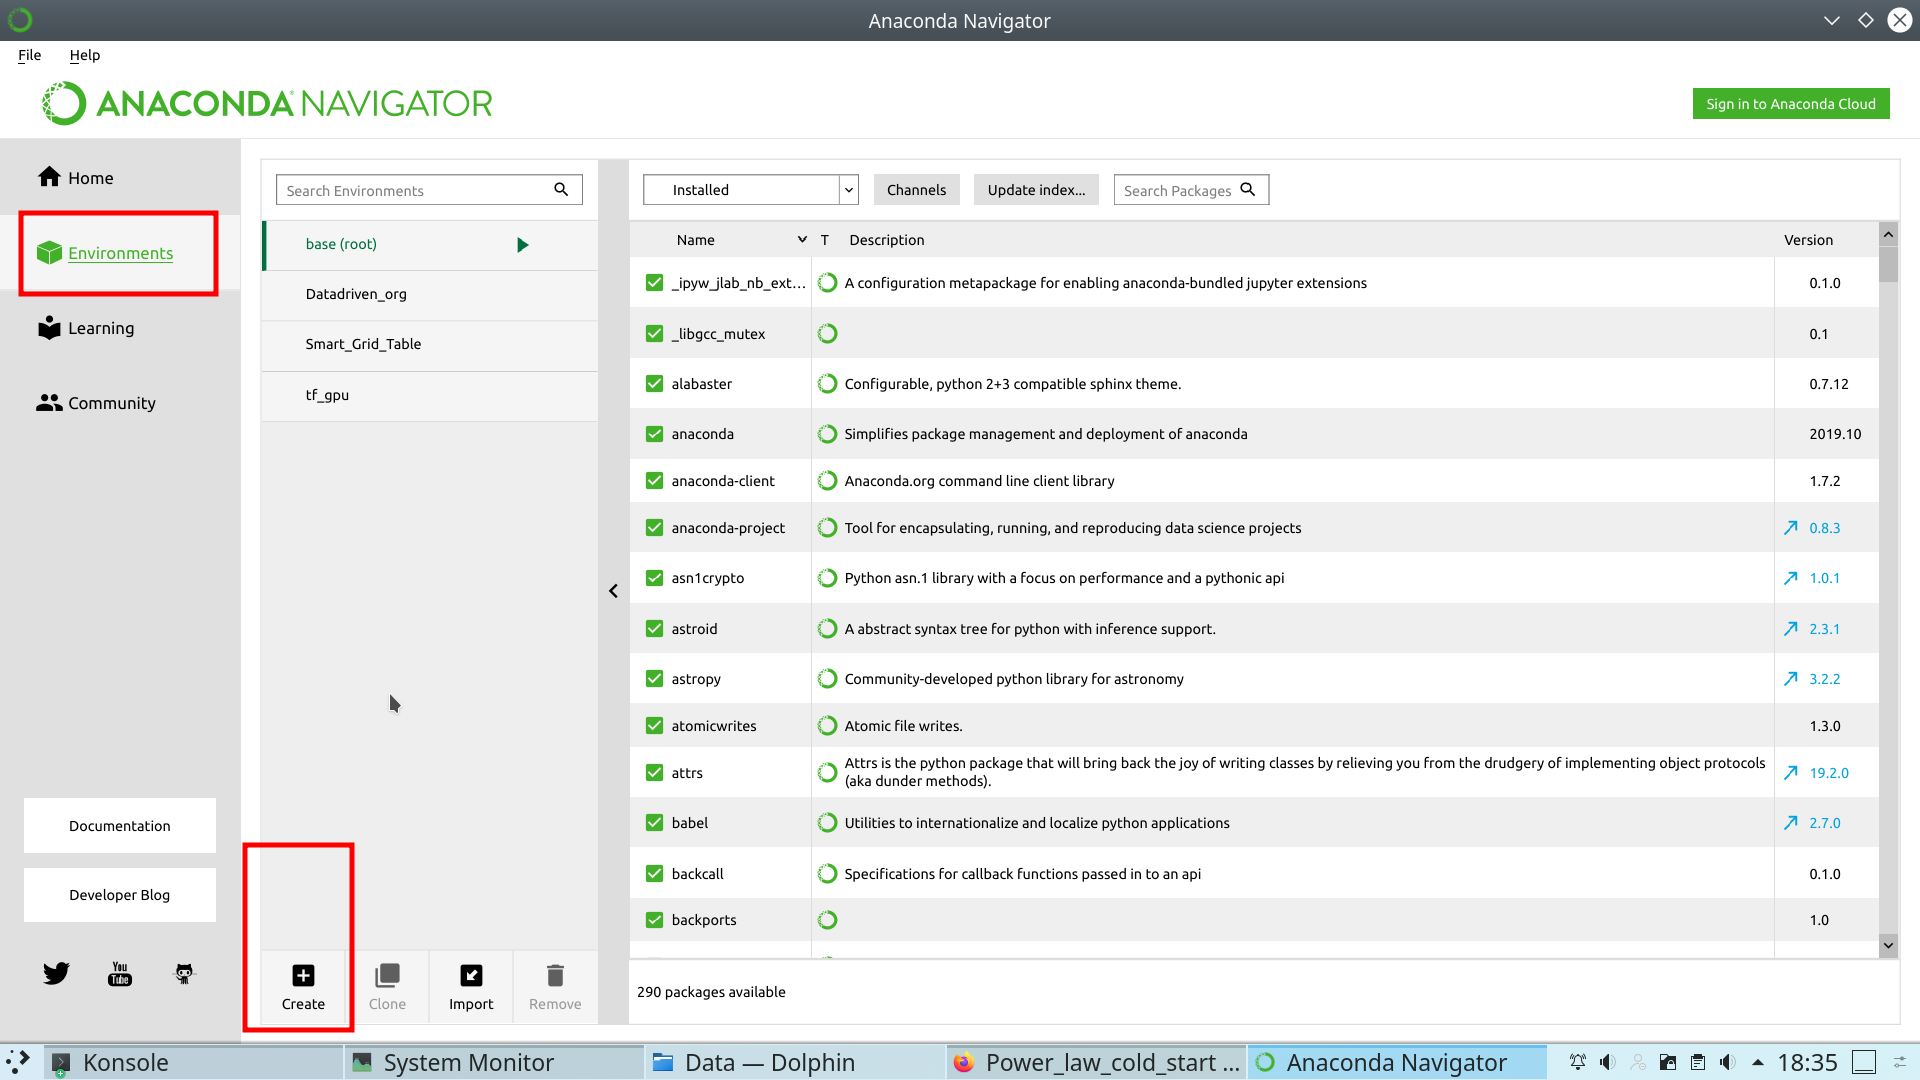
\includegraphics[width=1\columnwidth]{env.png}
\caption[Short title]{create environment}
\label{fig:ff2}\end{figure}


A few standard packages will be installed when creating a new environment. However, most of the useful packages (libraries) need to be installed manually.\\   
There are multiple way to install the missing packages.Search for the missing packages and install with anaconda-navigator. Look at instruction on pictures below:

\vspace{5mm}
\begin{figure}[H]
\centering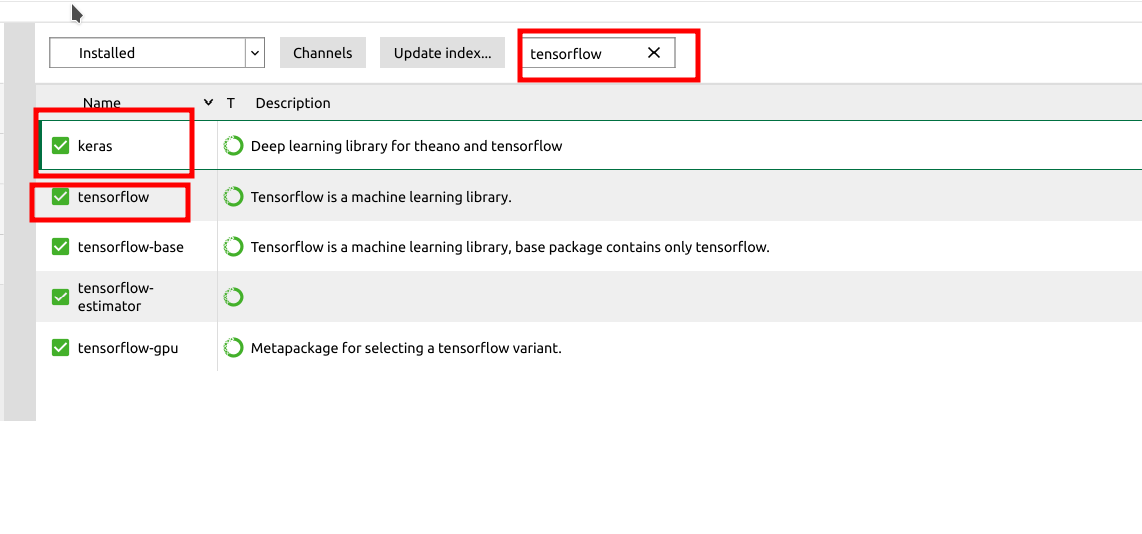
\includegraphics[width=1\columnwidth]{packages.png}
\caption[Short title]{install packages}
\label{fig:ff3}\end{figure}

\newpage

Installing packages with Console. Keep in mind that the virtual environment needs to be activated before installing the missing packages.

\begin{figure}[H]
\centering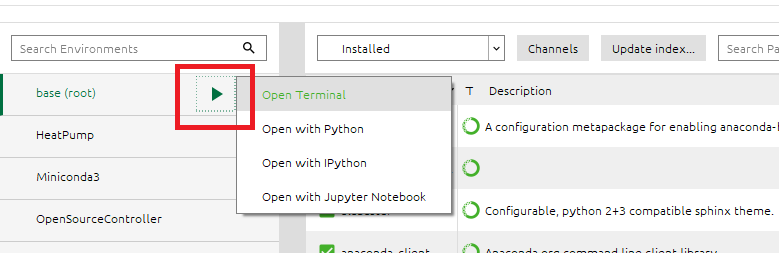
\includegraphics[width=1\columnwidth]{Open_terminal.png}
\caption[Short title]{Open terminal}
\label{fig:ff4}\end{figure}

\begin{figure}[H]
\centering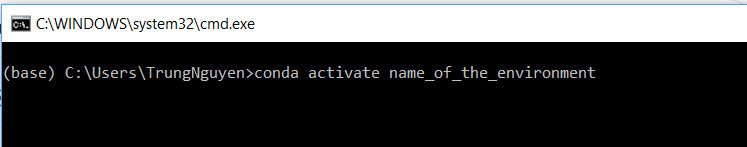
\includegraphics[width=1\columnwidth]{activate_env.png}
\caption[Short title]{Activate Environment}
\label{fig:ff5}\end{figure}

Find the missing packages from :\href{https://anaconda.org/conda-forge/repo}{Anaconda repo}.\\ 
Copy one of the command in the red box and paste to the terminal.

\begin{figure}[H]
\centering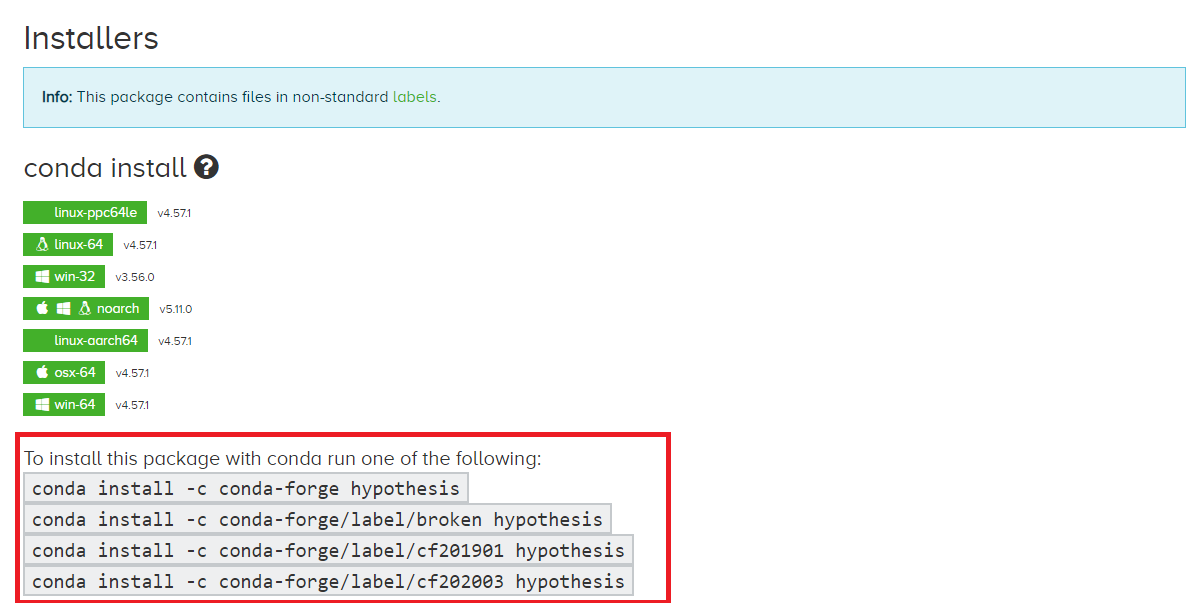
\includegraphics[width=1\columnwidth]{install_pack.png}
\caption[Short title]{Install package}
\label{fig:ff6}\end{figure}



\medskip

% ---------------------------------------------------------------------

\section{Getting started}
\label{sec:start}

The easiest way to get start is using a Jupyter notebook.
"The Jupyter Notebook is an open-source web application that allows you to create and share documents that contain live code, equations, visualizations and narrative text. Uses include: data cleaning and transformation, numerical simulation, statistical modeling, data visualization, machine learning, and much more." \cite{Jupyternotebook}.\\
There are several alternative online Jupyter note book available for free such as \href{https://colab.research.google.com/notebooks/welcome.ipynb}{Google Colab},\href{https://www.kaggle.com/}{Kaggle},...etc. The instruction on how to setup these online platform will be discusses in separate document.\\
Open Jupyter note book by click "Launch"

\begin{figure}[H]
\centering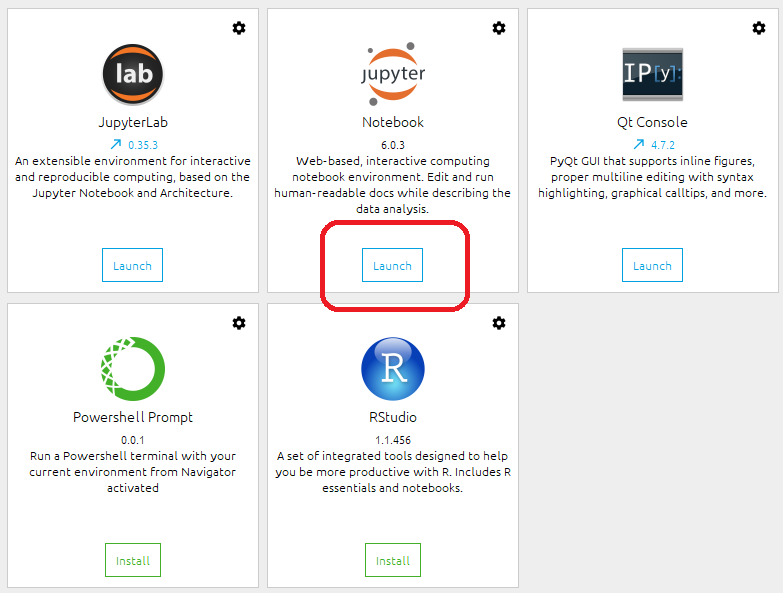
\includegraphics[width=1\columnwidth]{Jupyter.png}
\caption[Short title]{Open Jupyter notebook}
\label{fig:ff7}\end{figure}

\begin{figure}[H]
\centering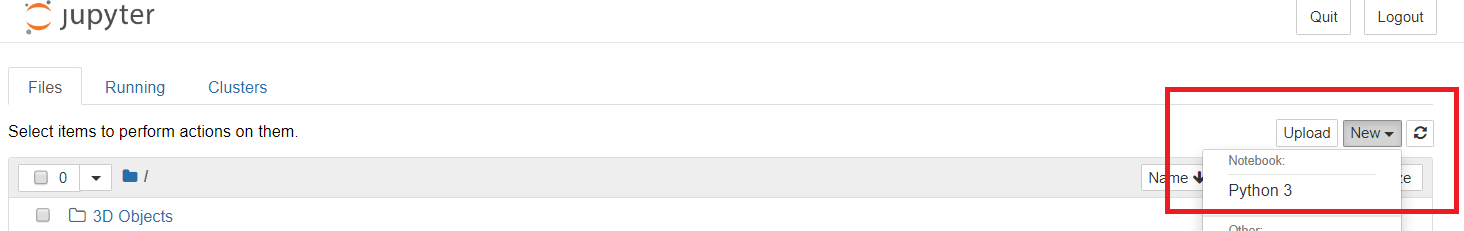
\includegraphics[width=1\columnwidth]{Jupyter_new.png}
\caption[Short title]{Create a new python 3 project}
\label{fig:ff8}\end{figure}

\vspace{1cm}

Now try to write something with Jupyter notebook and click Run button or "Shift-Enter"

\begin{figure}[H]
\centering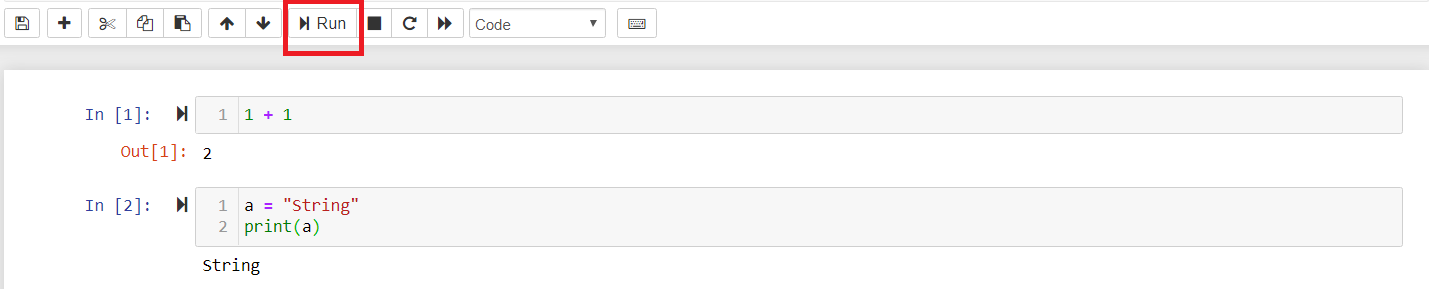
\includegraphics[width=1\columnwidth]{Jupyter_try.png}
\caption[Short title]{Simple example}
\label{fig:ff9}\end{figure}

\vspace{1cm}

Downloading \href{https://nbviewer.jupyter.org/github/jupyter/notebook/blob/master/docs/source/examples/Notebook/Running\%20Code.ipynb#}{Notebook example}. Click execute on Binder to try it online on your browser


\begin{figure}[H]
\centering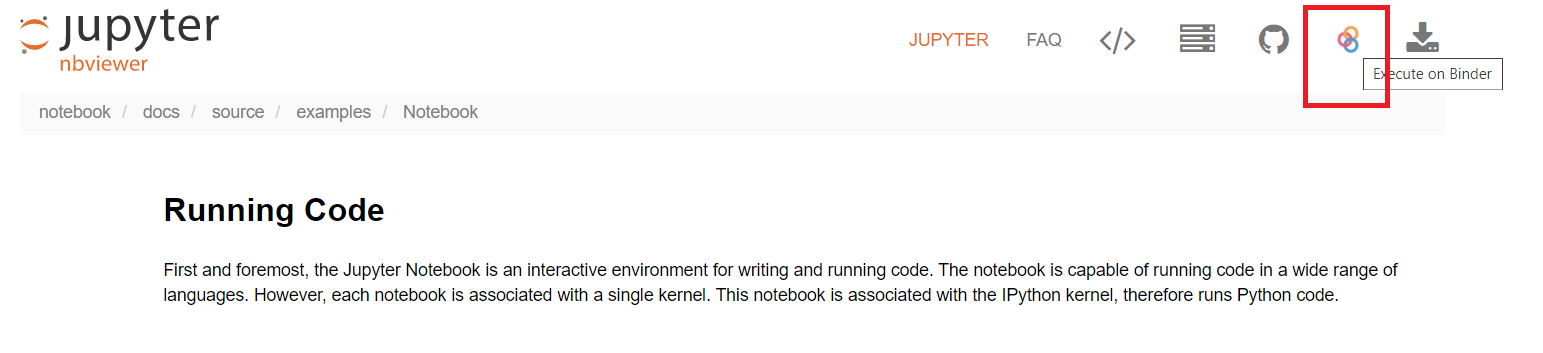
\includegraphics[width=1\columnwidth]{Jupyter_online_try.png}
\caption[Short title]{Online example}
\label{fig:ff10}\end{figure}

\vspace{1cm}

\href{https://github.com/jupyter/notebook/blob/master/docs/source/examples/Notebook/Running\%20Code.ipynb}{Github example folder}.\\
Using google search with key world "Jupyter notebook for beginner"

%---------------------------------------------------------

\section{Link to relevant information}

\hspace{3ex}\href{https://docs.anaconda.com/anaconda/user-guide/cheatsheet/}{Anaconda user guide cheatsheet}.

\href{https://docs.anaconda.com/anaconda/navigator/}{Navigator docs}


%-------------------------------------------------------------------------

\section{List of Documentation}

\begin{enumerate}
  \item Python Guideline for Beginner.
  \item Setting up Online Python Notebook
  \item update...
\end{enumerate}

\vspace{1cm}
\vspace{1cm}




%----------------------------------------------------------------

\section{Recommendation Courses}

\href{https://www.coursera.org/learn/machine-learning}{Machine learning by Andrew Ng.}\\
\href{https://www.usfca.edu/data-institute/certificates/deep-learning-part-one}{Deep Learning using FastAI  by Jeremy Howard.}


%----------------------------------------------------------------


%Bibliographic references
\printbibliography

\end{document}
